%input macros (i.e. write your own macros file called MacroFile1.tex)
%\include{Macros/MacroFile1}

\documentclass[oneside,12pt]{Classes/CUEDthesisPSnPDF}

\usepackage{tabularx}
\usepackage{rotating}
\usepackage{tikz}
\usepackage{listings}
\usepackage[acronym]{glossaries}







\ifpdf
%    \pdfinfo { /Title  (LIT Masters Thesis)
%               /Creator (TeX)
%               /Producer (pdfTeX)
%               /Author (Firstname Lastname K12345678@student.lit.ie)
%               /CreationDate (D:20120601000000)  %format D:YYYYMMDDhhmmss
%               /ModDate (D:20120615213532)
%               /Subject (LIT Masters Thesis)
%               /Keywords (PhD, Thesis)}
    \pdfcatalog { /PageMode (/UseOutlines)
                  /OpenAction (fitbh)  }
\fi

\title{LIT Masters Thesis Title}
\stitle{Subtitle of Thesis}
\supervisor{Supervisor}
\formalsupervisor{Dr. Super Visor}
\cosupervisor{Co-Supervisor}
\formalcosupervisor{Dr. Co Supervisor}
\formalauthor{Ms. Anne E. Mal}

\ifpdf
  \author{\href{mailto:k12345678@student.lit.ie}{Student Name}}
  \collegeordept{\href{https://lit.ie/aset/built-environment}{Department of the Built Environment}}
  \university{\href{http://www.lit.ie}{Limerick Institute of Technology}}
% insert below the file name that contains the crest in-place of 'UnivShield'
  \crest{
\includegraphics[width=90mm]{LITBuiltLogo.png}}

\else
  \author{Student Name}
  \collegeordept{Department of the Built Environment}
  \university{Limerick Institute of Technology}
% insert below the file name that contains the crest in-place of 'UnivShield'
  \crest{
\includegraphics[bb = 0 0 292 336, width=90mm]{LITBuiltLogo.jpg}}

\fi



%
% insert below the file name that contains the crest in-place of 'UnivShield'
% \crest{\IncludeGraphicsW{UnivShield}{40mm}{14 14 73 81}}
%
%\renewcommand{\submittedtext}{change the default text here if needed}
\degree{Master of Science}
\degreedate{Yet to be decided}

% turn of those nasty overfull and underfull hboxes
\hbadness=10000
\hfuzz=50pt

% Put all the style files you want in the directory StyleFiles and usepackage like this:
%\usepackage{StyleFiles/watermark}
%\usepackage{watermark}


% Comment out the next line to get single spacing
\onehalfspacing

\begin{document}

%\language{english}

% A page with the abstract on including title and author etc may be
% required to be handed in separately. If this is not so, then comment
% the below 3 lines (between '\begin{abstractseparte}' and 
% 'end{abstractseparate}'), normally like a declaration ... needs some more
% work, mind as environment abstracts creates a new page!
% \begin{abstractseparate}
%   \input{Abstract/abstract}
% \end{abstractseparate}




% Using the watermark package which is in StyleFiles/
% and to remove DRAFT COPY ONLY appearing on the top of all pages comment out below line
%\watermark{DRAFT COPY ONLY}


\maketitle

%set the number of sectioning levels that get number and appear in the contents
\setcounter{secnumdepth}{3}
\setcounter{tocdepth}{3}

\frontmatter % book mode only
\pagenumbering{roman}
\include{Declaration/declaration}
\include{Dedication/dedication}
\include{Acknowledgement/acknowledgement}
\include{Abstract/abstract}

\tableofcontents
\listoffigures
\printnomenclature  %% Print the nomenclature
\addcontentsline{toc}{chapter}{Nomenclature}

\mainmatter % book mode only
\include{Introduction/introduction}
% \pagebreak[4]
% \hspace*{1cm}
% \pagebreak[4]
% \hspace*{1cm}
% \pagebreak[4]

\chapter{My First Chapter But Note The Numbering ...}
\ifpdf
    \graphicspath{{Chapter1/Chapter1Figs/PNG/}{Chapter1/Chapter1Figs/PDF/}{Chapter1/Chapter1Figs/}}
\else
    \graphicspath{{Chapter1/Chapter1Figs/EPS/}{Chapter1/Chapter1Figs/}}
\fi
\markboth{\MakeUppercase{\thechapter. My First Chapter }}{\thechapter. My First Chapter}

\section{First Paragraph}

And now I begin my first chapter here ...

Here is an equation\footnote{the notation is explained in the nomenclature section :-)}:
\begin{eqnarray}
CIF: \hspace*{5mm}F_0^j(a) &=& \frac{1}{2\pi \iota} \oint_{\gamma} \frac{F_0^j(z)}{z - a} dz
\end{eqnarray}
\nomenclature[zcif]{$CIF$}{Cauchy's Integral Formula}                                % first letter Z is for Acronyms 
\nomenclature[aF]{$F$}{complex function}                                                   % first letter A is for Roman symbols
\nomenclature[gp]{$\pi$}{ $\simeq 3.14\ldots$}                                             % first letter G is for Greek Symbols
\nomenclature[gi]{$\iota$}{unit imaginary number $\sqrt{-1}$}                      % first letter G is for Greek Symbols
\nomenclature[gg]{$\gamma$}{a simply closed curve on a complex plane}  % first letter G is for Greek Symbols
\nomenclature[xi]{$\oint_\gamma$}{integration around a curve $\gamma$} % first letter X is for Other Symbols
\nomenclature[rj]{$j$}{superscript index}                                                       % first letter R is for superscripts
\nomenclature[s0]{$0$}{subscript index}                                                        % first letter S is for subscripts

\section{Second Paragraph}
and here I write more ...\cite{texbook}

\subsection{Compiler}

This template has been configured to work best with the pdfLatex compiler.  You may have to change some stuff to make it work with XeLatex.


\subsection{Mendeley}

Mendeley is not necessary for \LaTeX.  Mendeley is a standalone referencing management system that can be integrated to Microsoft Word or with \LaTeX.  The Mendeley application will manage your references in a manner similar to EndNote.  The major advantage of Mendeley is that it will also manage your downloaded .pdf files.  For more details of Mendeley and its functionality please go to \href{http://www.mendeley.com/}{www.mendeley.com} 





\subsection{MiKTeX}

The MiKTeX distribution contains the source files and executables for \LaTeX  to work.  The MiKTex distribution comes is available  from \href{http://miktex.org/}{miktex.org}  Please note that a completed installation will consume approx 2.0 Gig of hard disk space.  As the system is based on 'packages' you can elect to download and install packages as they are required.  This will substantially reduce the hard disk requirement; however it can pose problems when internet connectivity is lost.  My preferred option is to install the full distribution.  


\subsection{TeXstudio}

In order to use \LaTeX you will need a text editor.  There are numerous editors available for free download.  To date I have found TeXstudio to be the most flexible.  TeXstudio is available from  \href{https://www.texstudio.org/}{https://www.texstudio.org/} 






\subsection{Referencing and Citation}
... and some more ...

Now I would like to cite the following: \cite{latex} and \cite{texbook}
and \cite{Rud73}.

Referencing or citation can be achieved in a number of formats.  The standard is the \verb|\cite| command which will display as above.  Alternatives are \verb|\citet| and   \verb|\citep|.  The \verb|\citet| command produces \citet{KR83} whereas the \verb|\citep| command produces \citep{latex}.  More information is available from the  \href{http://merkel.zoneo.net/Latex/natbib.php}{Natbib Reference Sheet by Ross Moore}

\subsection{Including Figures and Pictures}


I would also like to include a picture ...

\begin{figure}[!htbp]
  \begin{center}
    \leavevmode
    \ifpdf
      \includegraphics[height=6in]{aflow}
    \else
      \includegraphics[bb = 92 86 545 742, height=6in]{aflow}
    \fi
    \caption{Airfoil Picture}
    \label{FigAir}
  \end{center}
\end{figure}

% above code has been macro-fied in Classes/MacroFile.tex file
%\InsertFig{\IncludeGraphicsH{aflow}{6in}{92 86 545 742}}{Airfoil Picture}{FigAir}

So as we have now labelled it we can reference it, like so (\ref{FigAir}) and it
is on Page \pageref{FigAir}. And as we can see, it is a very nice picture and we
can talk about it all we want and when we are tired we can move on to the next
chapter ...

I would also like to add an extra bookmark in acroread like so ...
\ifpdf
  \pdfbookmark[2]{bookmark text is here}{And this is what I want bookmarked}
\fi

% ------------------------------------------------------------------------


%%% Local Variables: 
%%% mode: latex
%%% TeX-master: "../thesis"
%%% End: 

\chapter{My Second Chapter}
\ifpdf
    \graphicspath{{Chapter2/Chapter2Figs/PNG/}{Chapter2/Chapter2Figs/PDF/}{Chapter2/Chapter2Figs/}}
\else
    \graphicspath{{Chapter2/Chapter2Figs/EPS/}{Chapter2/Chapter2Figs/}}
\fi

\markboth{\MakeUppercase{\thechapter. My Second Chapter }}{\thechapter. My Second Chapter}


\section{Some Standard things that you may need}

\subsection{Tables}

This subsection contains a few examples of tables such as table \ref{tab:TestTable} and table \ref{tab:StatusData}.  It also shows a use case for the tabularx environment shown in table \ref{tab:tabularx}.\\


\begin{table}[ht]
	\centering
	\begin{tabular}{|c|c|}
		\hline
		Item & Entry \\
		\hline
		Item  & Entry \\
		\hline
	\end{tabular}
	\caption{Table Name}
	\label{tab:TestTable}
\end{table}

\begin{table}[ht]
	\begin{tabularx}{\textwidth}{ |X|X| }
		\hline
		\textbf{Important stuff:} & As stated \\
		\hline 
		\textbf{More Important Stuff:}  & As stated  \\
		\hline
	
	\end{tabularx}
	\caption{tab:Using TabularX}
	\label{tab:tabularx}
\end{table}

\begin{table}[ht]
	\centering
	\begin{tabular}{ |c|r| }
		\hline
		\textbf{No.} & \textbf{Status Data} \\
		\hline 
		1 &  Some \\ 
		2 &  Data \\ 
		3 &  shown\\ 
		4 &  here \\
		\hline
	\end{tabular}
	\caption{Status Data}	
	\label{tab:StatusData}
\end{table}


\subsection{Figures}

Generally, images are pretty simple.  Use .jpg or png and you will be fine.  Just remember the captions.  If you need to rotate an image, you will have to do slightly more work.  All images here are licences under Creative Commons.

% TODO: \usepackage{graphicx} required
\begin{figure}[ht]
	\centering
	\includegraphics[width=0.7\linewidth]{./jpg/ColorfullSky.jpg}
	\caption[Colorfull Sky]{Colorful clouds and blue sky with water reflection of an island hosting trees at sunrise in Si Phan Don, Laos. Basile Morin, CC BY-SA 4.0}
	\label{fig:ColorSky}
\end{figure}


\begin{sidewaysfigure}[ht]
	\centering
	\includegraphics[width=1.0\linewidth]{./jpg/ColorfullSky.jpg}
	\caption{Sideways Image}
	\label{fig:SidewaysImage}
\end{sidewaysfigure}


\subsection{Vector Graphic Images}
Vector graphics can be handled in two ways.  Firstly, you can use eps files generated in another application, or secondly you can create the images on the fly using tikzpicture. A vector image is shown in figure \ref{fig:VennDiagram}.

\begin{figure}[ht]
	\centering
	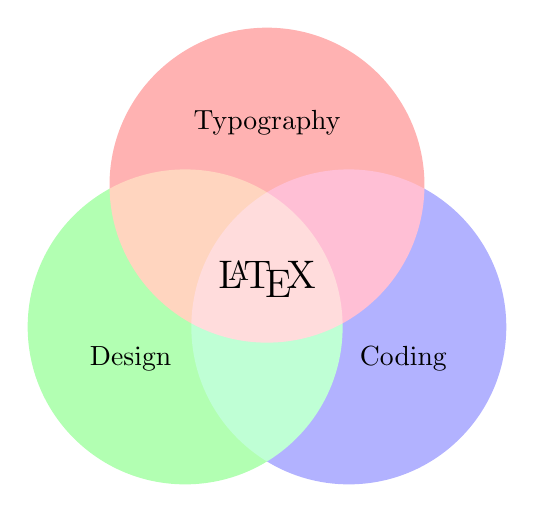
\begin{tikzpicture}
		\begin{scope}[blend group = soft light]
			\fill[red!30!white]   ( 90:1.2) circle (2);
			\fill[green!30!white] (210:1.2) circle (2);
			\fill[blue!30!white]  (330:1.2) circle (2);
		\end{scope}
		\node at ( 90:2)    {Typography};
		\node at ( 210:2)   {Design};
		\node at ( 330:2)   {Coding};
		\node [font=\Large] {\LaTeX};
	\end{tikzpicture}
	\label{fig:VennDiagram}
	\caption{More Vector examples from: \href{https://texample.net/tikz/examples/all/}{https://texample.net/tikz/examples/all/}}
\end{figure}

\newpage
\section{Computer Code}

\subsection{No Code Highlighting}
There are a few useful options for code also.  If you just want a simple listing, without code highlighting, then 'verbatium' is a good option.  You will have to convert tabs to 4 spaces.
\begin{verbatim}
def scope_test():
    def do_local():
        spam = "local spam"
	
    def do_nonlocal():
        nonlocal spam
        spam = "nonlocal spam"
	
    def do_global():
        global spam
        spam = "global spam"
	
    spam = "test spam"
    do_local()
    print("After local assignment:", spam)
    do_nonlocal()
    print("After nonlocal assignment:", spam)
    do_global()
    print("After global assignment:", spam)
	
    scope_test()
    print("In global scope:", spam)
\end{verbatim}


\subsection{Code Highlighting}

The Listings package will add code highlighting for you, but will not add color. The example shown is for Python; this can be changed to other languages by setting the language correctly.


\begin{lstlisting}[language=Python]
	import numpy as np
	
	def incmatrix(genl1,genl2):
	m = len(genl1)
	n = len(genl2)
	M = None #to become the incidence matrix
	VT = np.zeros((n*m,1), int)  #dummy variable
	
	#compute the bitwise xor matrix
	M1 = bitxormatrix(genl1)
	M2 = np.triu(bitxormatrix(genl2),1) 
	
	for i in range(m-1):
	for j in range(i+1, m):
	[r,c] = np.where(M2 == M1[i,j])
	for k in range(len(r)):
	VT[(i)*n + r[k]] = 1;
	VT[(i)*n + c[k]] = 1;
	VT[(j)*n + r[k]] = 1;
	VT[(j)*n + c[k]] = 1;
	
	if M is None:
	M = np.copy(VT)
	else:
	M = np.concatenate((M, VT), 1)
	
	VT = np.zeros((n*m,1), int)
	
	return M
\end{lstlisting}

The lstlisting environment can be customised to show color syntax highlighting, but it takes a bit of work and is specific to the language.  A good tutorial is here \href{https://denbeke.be/blog/programming/syntax-highlighting-in-latex/}{https://denbeke.be/blog/programming/syntax-highlighting-in-latex/}



\include{Chapter3/chapter3}
\include{Conclusions/conclusions}

\backmatter % book mode only

\bibliographystyle{agsm}
%\bibliographystyle{plainnat}
%\bibliographystyle{Classes/CUEDbiblio}
%\bibliographystyle{Classes/jmb}
%\bibliographystyle{Classes/jmb} % bibliography style
\renewcommand{\bibname}{References} % changes default name Bibliography to References
\bibliography{References/references} % References file

\appendix
%\setcounter{page}{1}

\include{Appendix1/appendix1}
\chapter{Appendix B}
\setcounter{page}{1}
\renewcommand{\thepage}{B-\arabic{page}}
\markboth{\MakeUppercase{Appendix B }}{Appendix B}

Look again at that dot. That's here. That's home. That's us. On it everyone you love, everyone you know, everyone you ever heard of, every human being who ever was, lived out their lives. The aggregate of our joy and suffering, thousands of confident religions, ideologies, and economic doctrines, every hunter and forager, every hero and coward, every creator and destroyer of civilization, every king and peasant, every young couple in love, every mother and father, hopeful child, inventor and explorer, every teacher of morals, every corrupt politician, every "superstar," every "supreme leader," every saint and sinner in the history of our species lived there--on a mote of dust suspended in a sunbeam.

Let's light this fire one more time, Mike, and witness this great nation at its best.

It's just mind-blowingly awesome. I apologize, and I wish I was more articulate, but it's hard to be articulate when your mind's blown, but in a very good way.

I am a stranger. I come in peace. Take me to your leader and there will be a massive reward for you in eternity.

We choose to go to the moon. We choose to go to the moon in this decade and do the other things, not because they are easy, but because they are hard, because that goal will serve to organize and measure the best of our energies and skills, because that challenge is one that we are willing to accept, one we are unwilling to postpone, and one which we intend to win, and the others, too.

That's one small step for [a] man; one giant leap for mankind.

The size and age of the Cosmos are beyond ordinary human understanding. Lost somewhere between immensity and eternity is our tiny planetary home. In a cosmic perspective, most human concerns seem insignificant, even petty. And yet our species is young and curious and brave and shows much promise. In the last few millennia we have made the most astonishing and unexpected discoveries about the Cosmos and our place within it, explorations that are exhilarating to consider. They remind us that humans have evolved to wonder, that understanding is a joy, that knowledge is prerequisite to survival. I believe our future depends powerfully on how well we understand this Cosmos in which we float like a mote of dust in the morning sky.

The Earth is a very small stage in a vast cosmic arena. Think of the rivers of blood spilled by all those generals and emperors so that, in glory and triumph, they could become the momentary masters of a fraction of a dot. Think of the endless cruelties visited by the inhabitants of one corner of this pixel on the scarcely distinguishable inhabitants of some other corner, how frequent their misunderstandings, how eager they are to kill one another, how fervent their hatreds.

Houston, that may have seemed like a very long final phase. The autotargeting was taking us right into a ... crater, with a large number of big boulders and rocks ... and it required ... flying manually over the rock field to find a reasonably good area.

First, I believe that this nation should commit itself to achieving the goal, before this decade is out, of landing a man on the moon and returning him safely to the earth. No single space project in this period will be more impressive to mankind, or more important for the long-range exploration of space; and none will be so difficult or expensive to accomplish.

I saw for the first time the earth's shape. I could easily see the shores of continents, islands, great rivers, folds of the terrain, large bodies of water. The horizon is dark blue, smoothly turning to black. . . the feelings which filled me I can express with one word - joy.

A good rule for rocket experimenters to follow is this: always assume that it will explode.

It has been said that astronomy is a humbling and character-building experience. There is perhaps no better demonstration of the folly of human conceits than this distant image of our tiny world. To me, it underscores our responsibility to deal more kindly with one another, and to preserve and cherish the pale blue dot, the only home we've ever known.

The surface is fine and powdery. I can kick it up loosely with my toe. It does adhere in fine layers, like powdered charcoal, to the sole and sides of my boots. I only go in a small fraction of an inch, maybe an eighth of an inch, but I can see the footprints of my boots and the treads in the fine, sandy particles. There seems to be no difficult in moving around, as we suspected.

From this day forward, Flight Control will be known by two words: 'Tough' and 'Competent.' Tough means we are forever accountable for what we do or what we fail to do. We will never again compromise our responsibilities. Every time we walk into Mission Control we will know what we stand for. Competent means we will never take anything for granted. We will never be found short in our knowledge and in our skills. Mission Control will be perfect. When you leave this meeting today you will go to your office and the first thing you will do there is to write 'Tough and Competent' on your blackboards. It will never be erased. Each day when you enter the room these words will remind you of the price paid by Grissom, White, and Chaffee. These words are the price of admission to the ranks of Mission Control.

The view of the Earth from the Moon fascinated me, small disk, 240,000 miles away. It was hard to think that that little thing held so many problems, so many frustrations. Raging nationalistic interests, famines, wars, pestilence don't show from that distance.

The Earth is the only world known so far to harbor life. There is nowhere else, at least in the near future, to which our species could migrate. Visit, yes. Settle, not yet. Like it or not, for the moment the Earth is where we make our stand.

Our posturings, our imagined self-importance, the delusion that we have some privileged position in the Universe, are challenged by this point of pale light. Our planet is a lonely speck in the great enveloping cosmic dark. In our obscurity, in all this vastness, there is no hint that help will come from elsewhere to save us from ourselves.

The vehicle explodes, literally explodes, off the pad. The simulator shakes you a little bit, but the actual liftoff shakes your entire body and soul.



% ------------------------------------------------------------------------

%%% Local Variables: 
%%% mode: latex
%%% TeX-master: "../thesis"
%%% End: 








\end{document}
